Before we dive in into the specifics, we first will showcase the final architecture in the
Elastic Container Service (ECS), which is a fully managed container orchestration service,
more information about the ECS can be found in the following link \cite{ecs_intro}

\begin{figure}[!ht]
    \centering
    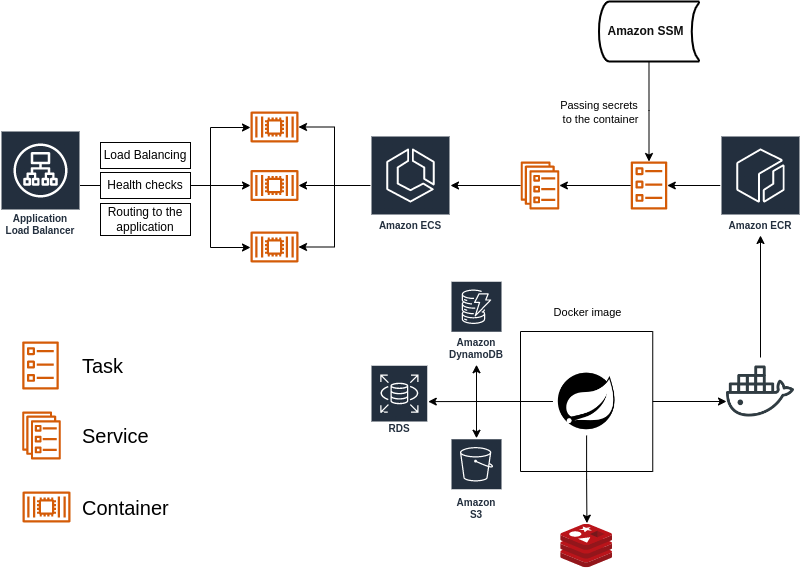
\includegraphics[width=\textwidth]{images/ECS}
    \caption{\footnotesize{ECS Architecture}}
    \label{fig:ECSArch}
\end{figure}

Task: the component which takes care of running the containers.

Service: the component which manages the tasks.

Container: the image that is running on the task.

\subsection {ECS Containerization and secrets}

The ECS solution shown in figure \ref{fig:ECSArch} was a bit of a challenge to get it to
work, as it was a containerized solution, and not a native one.
So the first step was to containerize the solution, and have a safe image that doesn't
expose any secrets or environment variables.

In the docker way, we can just pass them through the command line,
and the solution will run perfectly.

But here relied a problem that was the ECS solution, it didn't have a simple
way to feed it the credentials, environment variables neither files, so we had to opt
for using the SSM or Secrets Manager
which is yet another hosted solution to store strings as secrets, and then those could be 
passed to the ECS services.

With the Secrets Manager, for the strings secrets it was a simple writing / reading process
to store and retrieve the secrets. But for the files it was a bit more complicated, there
wasn't a direct way to do that.

Finally we came up with the following solution, which is as follows:

\begin{itemize}
    \item Serialize the content of the file into a base64 string
    \item Store the base64 string in the AWS Systems Manager (SSM)
    \item Pass the SSM secret to the ECS service
    \item Retrieve the secret from the SSM as a environment variable
    \item Decode the base64 string
    \item Store the deserialized base64 in a file in the container
    \item Point an environment variable to the file
\end{itemize}

As such we managed to pass aws credentials, google credentials and Redis Labs credentials.

\subsection {Load Balancer and routing}

As shown in the ECS Architecture, we had a load balancer in front of the running tasks, which has four main goals:

\begin{itemize}
    \item To take care of the incoming traffic from the client side
    \item To ensure that the traffic distributed evenly
    \item To ensure that the tasks are healthy
    \item To ensure that the tasks are not overloaded and manage it's scalability.
\end{itemize}

\begin{figure}[!htbp]
    \centering
    \includegraphics[width=\textwidth]{images/loadBalancer.png}
    \caption{\footnotesize{Load Balancer Interaction with the backend}}
    \label{fig:loadbalancer}
\end{figure}

So the load balancer is as shown in figure \ref{fig:loadbalancer}, it took traffic from
port 80 where it had an exposed dns link, then it routed it through a VPS to the
containers that are exposing post 8080 in their local network, having healthchecks
done on the endpoint /actuator/health .

With that set in place, we had pretty much everything setup to start testing for the
load handling by the ecs to check for the health of the containers and the measures
to be set to ensure that the auto scaling is setup with the right parameters.

So first, we written scripts that did kind of overload the server with the requests,
asynchronously deploy the containers and check monitoring metrics.

\begin{figure}[!ht]
    \centering
    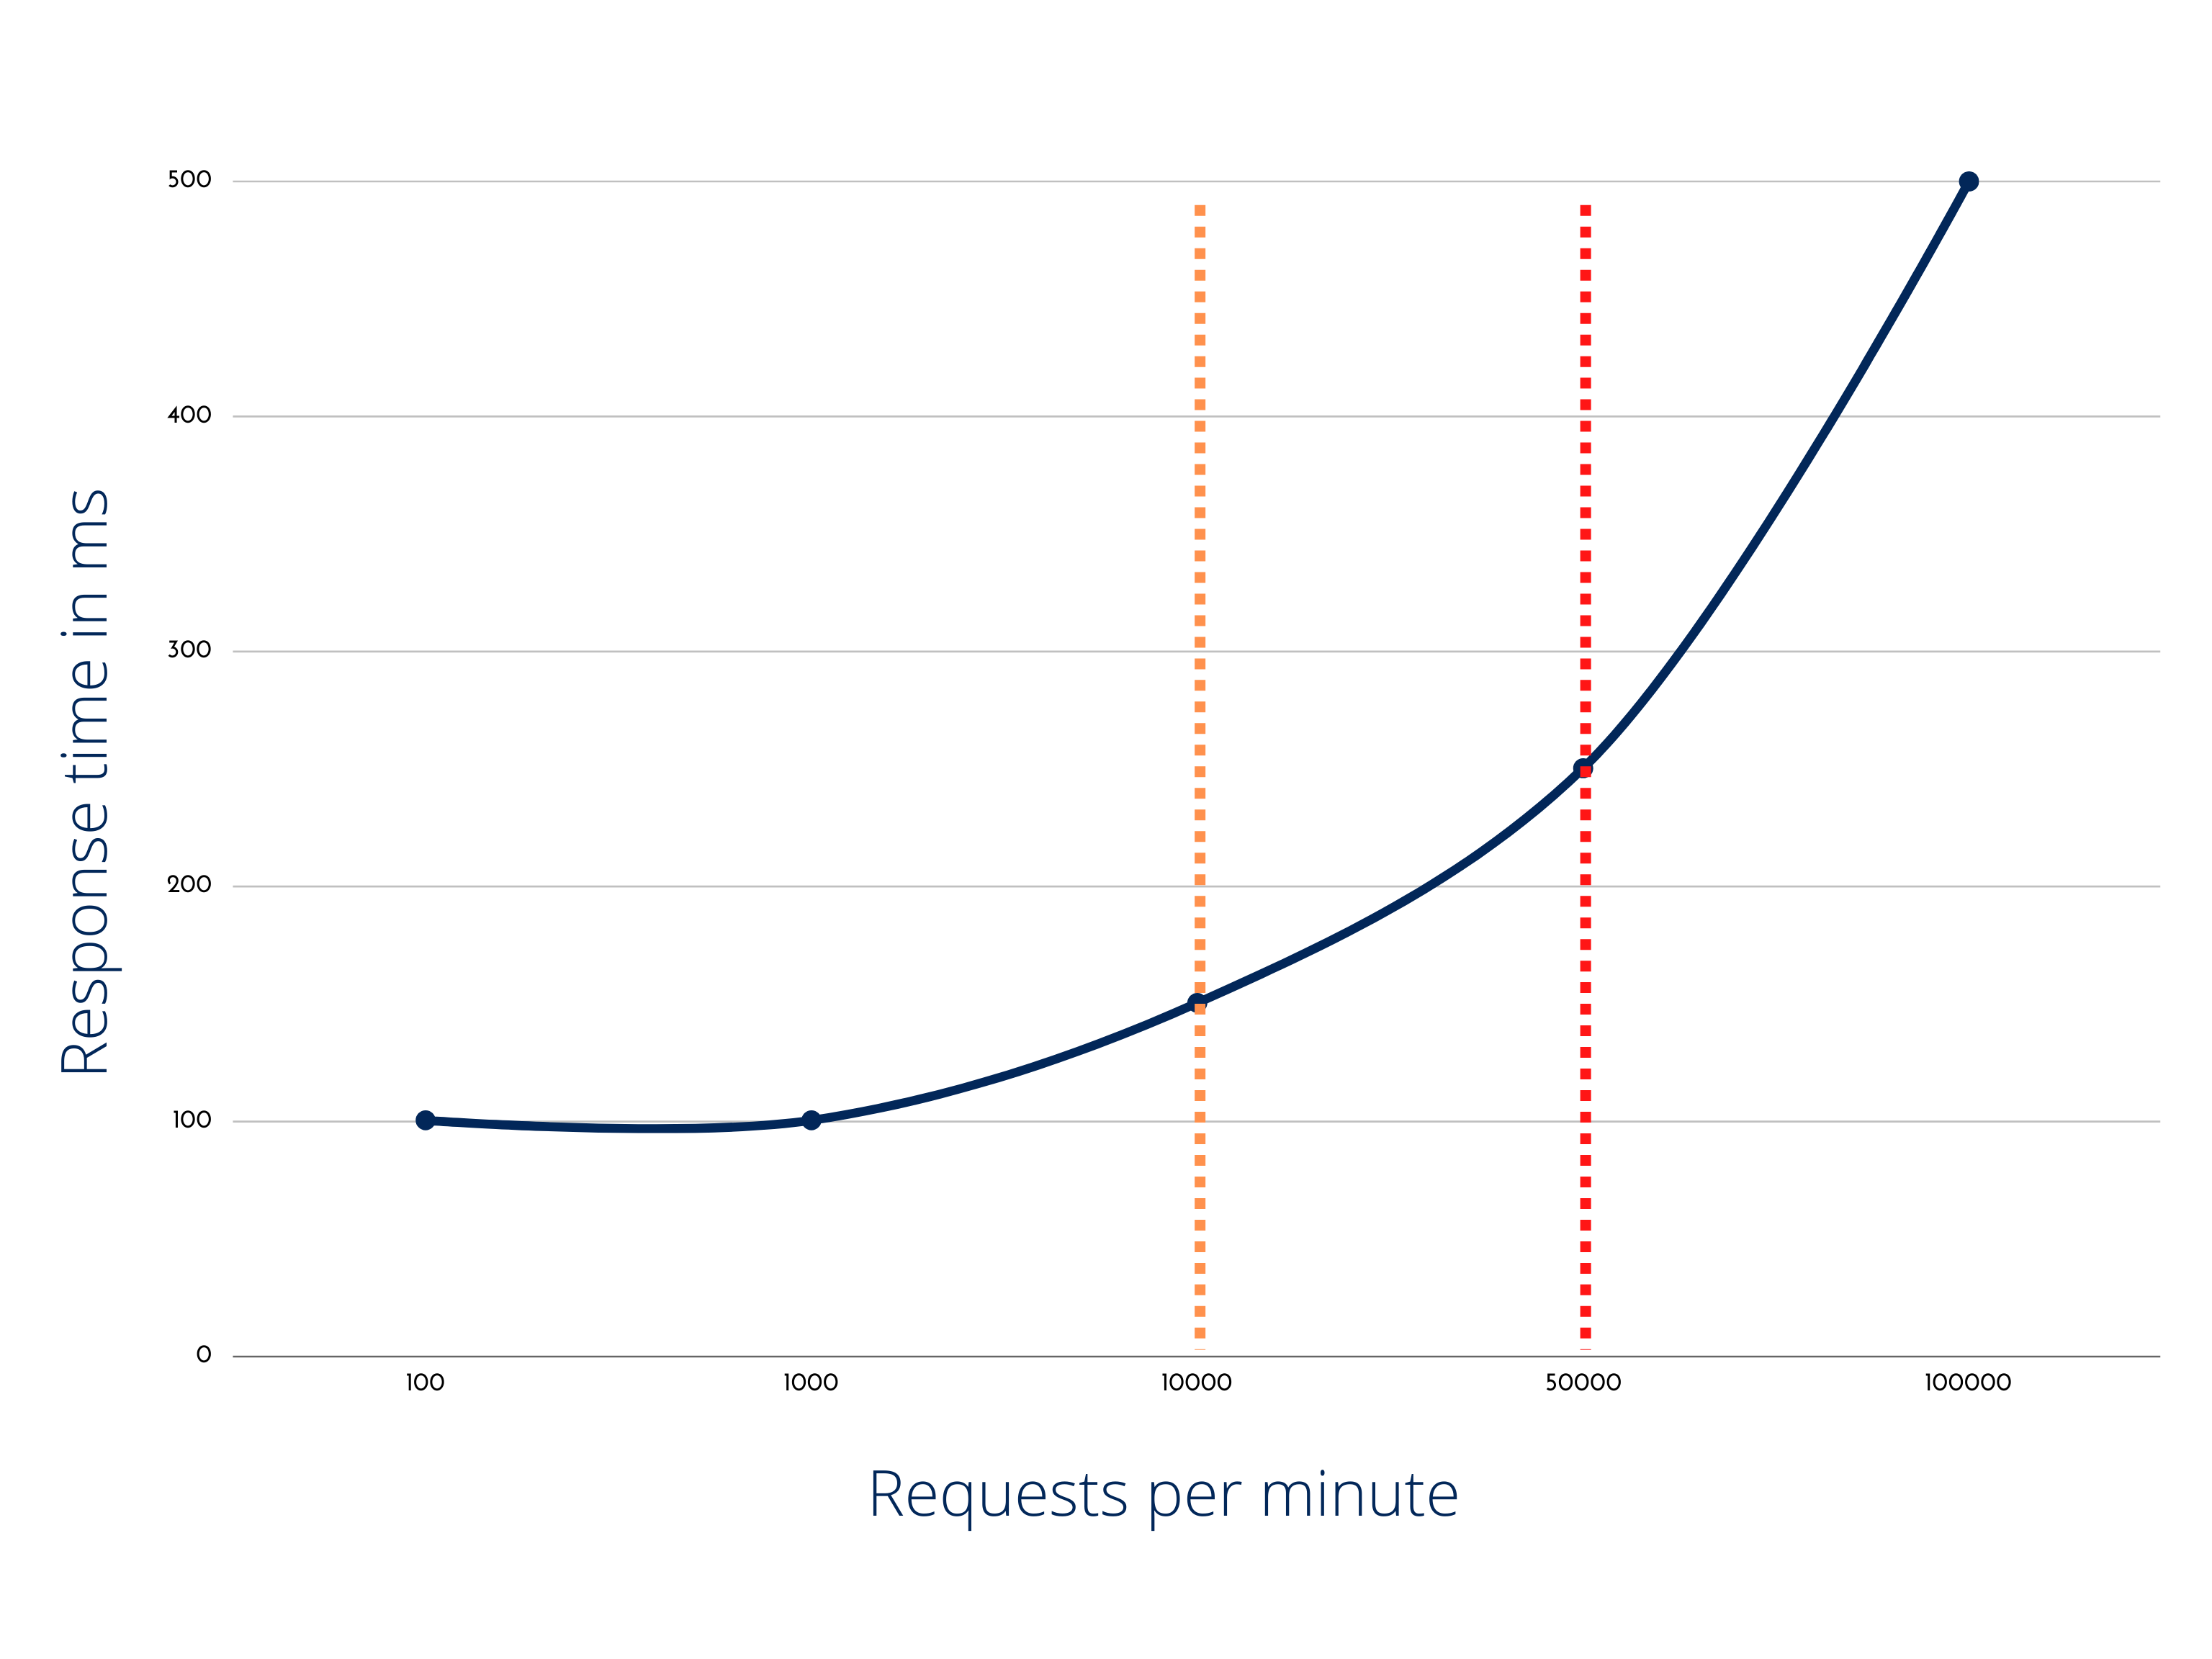
\includegraphics[width=\textwidth]{images/assesment_autoscaling.png}
    \caption{\footnotesize{Auto Scaling Assessment}}
    \label{fig:autoscaling_assessment}
\end{figure}

So next came doing the assessment of autoscaling, we ended up compiling the chart
in figure \ref{fig:autoscaling_assessment} which shows the response time per
number of requests sent per minute, the assesment was done by using a script
written in Scala.
Looking at the chart we can see that the response time was pretty stable until
we reached the 10000 requests mark, where there was a clear increase but nothing
that could kill the usage till we exceeded the 50000 mark where the response time
was getting really high meaning that at this point there's no advantage on keeping
only the existing instances up but the need to increase becomes apparent, and that
was due to the heavy requests creating a sort of queue in the backend which would
require multiple processes thus comes the horizontal increase advantage in the ECS.

So firstly, as shown in \ref{fig:loadtest} it took the endpoint to be hit, in case
it was a private endpoint you'd need to provide the credentials to. Then put in place
the number of requests to be sent and finally run it.

Once it started running it was a simple case of sending requests asynchronously in fibers
or virtual threads, and then printing the response time of each request, as such we could
monitor the handling time of the requests being affected by the load of requests.

\begin{figure}[!ht]
    \centering
    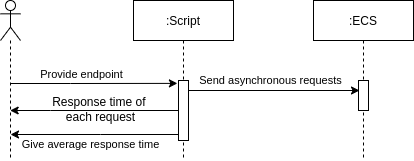
\includegraphics[width=0.8\textwidth]{images/scriptdos.png}
    \caption{\footnotesize{Load Test Script}}
    \label{fig:loadtest}
\end{figure}


Thus it we could find the right parameters for the autoscaling, based on the number of
requests being sent per minute, which at the time of tests was around 50000 requests per
minute without the response time being affected which is quite impressive.

And as most the back-end services relying heavily on the memory, we ensured to put a 70\%
memory usage limit on the containers before spawning new instances to handle the load, in
case of autoscaling by memory.

Next came the assesment and benchmarking of two databases solutions which were a Redis
instance hosted in EC2, and a Redislabs hosted instance.

The tests were done by using a script that was written in python, and it was a
stress testing script, which sole purpose was to overload the Redis instance 
and then check if the requests then took longer to fulfill, as Redis was a in-memory
database, so the goal of using it was speed.

\begin{table}[!ht]
    \centering
    \begin{tabular}{| c | c |}
        \hline
        \textbf{Database} & \textbf{Stress Test} \\
        \hline
        Redis on EC2 & 
                \begin{tabular}{| c | c |}
                    \textbf{Load} & \textbf{Response by Endpoint} \\
                    \hline
                    \textbf{25\%} &
                            \begin{tabular}{| c | c |}
                                \textbf{Endpoint} & \textbf{Response Time} \\
                                \hline
                                Add client & \textbf{129.9} \\
                                \hline
                                Get all clients & \textbf{89.9} \\
                                \hline
                                Heavy Load Enpoint & \textbf{269.2} \\
                            \end{tabular}\\
                    \hline
                    \textbf{50\%} &
                            \begin{tabular}{| c | c |}
                                \textbf{Endpoint} & \textbf{Response Time} \\
                                \hline
                                Add client & \textbf{128.3} \\
                                \hline
                                Get all clients & \textbf{106.1} \\
                                \hline
                                Heavy Load Enpoint & \textbf{245.7} \\
                            \end{tabular}\\
                    \hline
                    \textbf{75\%} &
                            \begin{tabular}{| c | c |}
                                \textbf{Endpoint} & \textbf{Response Time} \\
                                \hline
                                Add client & \textbf{133.6} \\
                                \hline
                                Get all clients & \textbf{196.1} \\
                                \hline
                                Heavy Load Enpoint & \textbf{257.7} \\
                                \hline
                            \end{tabular}\\
                \end{tabular}\\
        \hline
        Redis on RedisLab & 
                \begin{tabular}{| c | c |}
                    \textbf{Load} & \textbf{Response by Endpoint} \\
                    \hline
                    \textbf{25\%} &
                            \begin{tabular}{| c | c |}
                                \textbf{Endpoint} & \textbf{Response Time} \\
                                \hline
                                Add client & \textbf{154.1} \\
                                \hline
                                Get all clients & \textbf{79.5} \\
                                \hline
                                Heavy Load Enpoint & \textbf{256.8} \\
                            \end{tabular}\\
                    \hline
                    \textbf{50\%} &
                            \begin{tabular}{| c | c |}
                                \textbf{Endpoint} & \textbf{Response Time} \\
                                \hline
                                Add client & \textbf{134.1} \\
                                \hline
                                Get all clients & \textbf{126.4} \\
                                \hline
                                Heavy Load Enpoint & \textbf{241.2} \\
                            \end{tabular}\\
                    \hline
                    \textbf{75\%} &
                            \begin{tabular}{| c | c |}
                                \textbf{Endpoint} & \textbf{Response Time} \\
                                \hline
                                Add client & \textbf{143.5} \\
                                \hline
                                Get all clients & \textbf{156.3} \\
                                \hline
                                Heavy Load Enpoint & \textbf{258.2} \\
                                \hline
                            \end{tabular}\\
                \end{tabular}\\
        \hline
    \end{tabular}
    \caption{\footnotesize{Stress testing Redis against RedisLab}}
    \label{tab:stress_testing}
\end{table}

The results on the table above were quite impressive, as the response time of the
requests was quite low, and the load was quite high, the only noticeable growth was
in the response time of the Get All Clients and that was due to the fact that to 
increase the load on the Redis instance we had to increase the number of clients.
Thus, get all clients got heavier and heavier to handle.

As shown in \ref{tab:stress_testing}, it ended up being with a pretty close result,
no one over ruling the other, and the results were pretty close to the expected results.
So we ended up either having to opt for the Redis instance hosted in EC2 and do 
all the configuration manually which would lead to a lot of configuration done manually,
or just resorting to the Redislabs hosted instance, as it's a fully managed instance.
All the security measures and replication are taken care of by cloud host.

\subsection{Deployment}

Finally after testing everything, and having deployed one ECS service succesfully, we had
to automate the deployment process, so that we could handle new versions and code update
without much effort.

This came in the form of a gradle task, which was as follows:

    \begin{figure}[!htbp]
        \centering
        
\includegraphics[width=\textwidth]{images/gradle.png}
        \caption{\footnotesize{Deployment of the App to ECS - Gradle Task}}
        \label{fig:gradle}
    \end{figure}

The dockerization part of the gradle task was handled using a third party plugin,
then the deployment to Elastic Container Registry (ECR\footnote{ECR is an AWS managed
    container image registry service that is secure, scalable, and reliable. More
    information can be found in \cite{ecr_intro}.})e using the AWS CLI,
by linking the ECR to docker, then pushing the image is automatically uploaded to ECR.
Once this is done, the ECS service has to handle the update of the image, 
and this was done through a bash script that took in charge of getting a list 
of the running tasks, then stopping one of them, and wait for a new one to spawn 
such as to avoid down time during the update of the service.

    \begin{figure}[!ht]
        \centering
        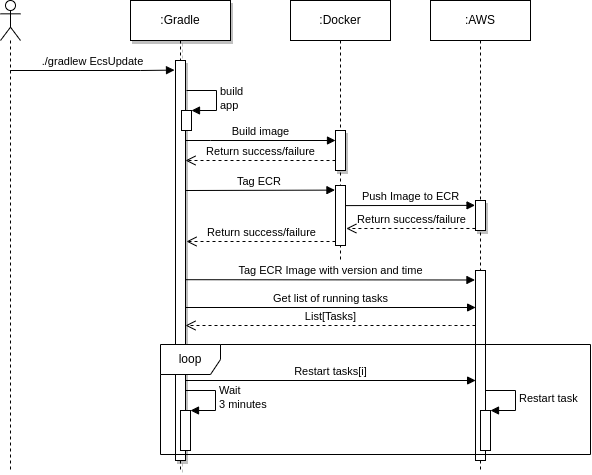
\includegraphics[width=0.9\textwidth]{images/gradleTask.png}
        \caption{\footnotesize{Deployment Sequence Diagram}}
        \label{fig:deployment}
    \end{figure}

So in the figure \ref{fig:deployment}, the flow is pretty simple,
it goes as follows:

    \begin{itemize}
        \item Gradle builds the docker image using a 3rd party plugin
        \item Tag image with right version of the application and push it to ECR
        \item Tag ECR image with current version in addition to timestamp it
        \item Get the list of running tasks
        \item Stop one of the running tasks
        \item Wait for a new one to spawn
        \item The two last steps are repeated till the list is exhausted
    \end{itemize}

And in such a way, we can handle the deployment without having any downtime,
so it makes introducing bug fixes a better experience for both developer and 
customer.

